\documentclass[12pt,letterpaper]{article}
\usepackage[utf8]{inputenc}
\usepackage[total={18cm,21cm},top=2cm, left=2cm]{geometry} 
\usepackage{amsmath,amssymb,amsfonts,latexsym} 
\usepackage{graphicx} %gràficos y figuras
\usepackage{caption}
\usepackage{dsfont}
\usepackage{multicol}
\usepackage{color, xcolor}
\usepackage{hyperref}
\usepackage{float}
\definecolor{amarilloclaro}{RGB}{238,243,144}
\definecolor{azulclaro}{RGB}{210,243,243}
%\pagestyle{empty} %Elimina la numeración de las páginas
\parskip=0.5cm %Genera un espacio de 0.5cm entre los párrafos
\parindent=0mm %Elimina la sangría.
\renewcommand{\tablename}{Tabla}
\renewcommand{\figurename}{Figura}
\renewcommand{\refname}{Bibliografía}
\renewcommand{\abstractname}{Resumen}
%\spanishdecimal{.}
%nuevos comandos
\newcommand{\R}{\mathds{R}}
\newcommand{\sen}{\text{sen}}
\newcommand{\limite}[2] { \lim_{ #1 \rightarrow #2}}
\newcommand{\abs}[1]{\left| #1 \right|}
\newcommand{\norma}[1]{\left\| #1 \right\|}
\newcommand{\raiz}[3]{\sqrt{{#1}^2+{#2}^2+{#3}^2}}
%%
%Paquete Tikz
\usepackage{tikz}
\usepackage{pgfplots}
\pgfplotsset{compat=1.8}
\tikzset{flechaizq/.style={<-,>=latex}} 
\tikzset{flechader/.style={->,>=latex}}
\tikzset{flechadoble/.style={<->,>=latex}}
\tikzset{punteada/.style={line width=2, dash pattern = on 6pt off 3pt}}
\tikzset{continua/.style={line width=1, flechadoble}}
\tikzset{conector/.style={line width=2, flechadoble, dashed}}
\usetikzlibrary{shapes}
\usetikzlibrary{positioning}
\usetikzlibrary{intersections}
%%
\title{Semillero de Investigación en Ecuaciones Diferenciales Ordinarias con Python}
\author{Jackeline Rivera Aguilera,\\
Milton Pablo Arias Rincón, \\
Daniel Felipe Franco Rincón,\\
David Rincón Toro,\\
Over.
\\\\
Asesor:\\
Luis Eduardo López-Montenegro, PhD.
}

\date{}

\begin{document}
\maketitle
\begin{abstract}
 Aqui se escribe un resumen del trabajo  
\end{abstract}

\section{Ecuaciones diferenciales ordinarias}
Una ecuación diferencial es una relación de igualdad entre dos expresiones algebraicas que contienen: derivadas, variables independientes, una variable dependiente y/o constantes (parámetros).

Si la ecuación diferencial tiene una sola variable independiente, se llama {\it Ecuación Diferencial Ordinaria} (EDO) y si tiene más de una variable independiente, se llama {\it Ecuación Diferencial Parcial} (EDP). De acuerdo al orden de su derivada, las ecuaciones diferenciales se clasifican en {\it primer orden} u {\it orden superior}.

Por ejemplo, 
\begin{itemize}
    \item $\displaystyle r \frac{dr}{d\theta} + \sen \theta = r^2 $, es una EDO de primer orden donde $\theta$ es la variable independiente y $r$ es la variable dependiente.
    \item $\displaystyle \frac{\partial z}{\partial x} + \left(\frac{\partial z}{\partial y}\right)^2=xz$, es una EDP de primer orden no lineal donde: $x,y$ son variables independientes, y $z$ es la variable dependiente.
    \item $t^2 x'' - tx' = 1$, es una EDO de segundo orden (orden superior) con variable independiente $t$ y variable dependiente $x$.
\end{itemize}

Una EDO de primer orden con variable independiente $t$ y variable dependiente $x$, se puede reescribir de la forma:
\begin{equation}\label{edo1}
    x'=f(t,x)
\end{equation}
Si $f(t,x)$ no depende de $t$, la EDO \eqref{edo1} se llama {\it EDO autónoma}. De lo contrario, se llama {\it no autónoma}.

La {\it solución general} de \eqref{edo1} es una familia de curvas $\psi(t,x,c)=0$, donde $c\in\R$, la cual satisface la ecuación \eqref{edo1}. Si $\psi_0(t,x,c_0)=0$ es una solución de \eqref{edo1} y además pasa por el punto $(t_0,x_0)$, $\psi_0$ se llama {\it solución particular} y satisface el {\it Problema de Valor Inicial} (PVI):
\begin{align}\label{pvi}
    & x'=f(t,x)\\ \nonumber
    & x(t_0)=x_0 
\end{align}

Este semillero se enfoca en el estudio de las EDO de primer orden mediante la aproximación numérica a la solución particular $\psi_0(t,x,c_0)=0$ del PVI \eqref{pvi} implementando {\it métodos numéricos} para resolver EDO implementados en el software Python, siguiendo la condiciones establecidas en el {\it Teorema de Existencia y Unicidad}.

{\bf Teorema de Existencia y Unicidad}. El PVI \eqref{pvi} tiene una \textbf{única} solución si, para un intervalo $I\subseteq\R^2$ que contiene al punto $(t_0, x_0)$, la EDO \eqref{edo1} satisface que:
\[
    f(t, x) \quad \text{y} \quad \frac{\partial f}{\partial x}, 
\]
son continuas en $I$ \cite[pp. 43]{librozill}

Es importante destacar que el cumplimiento de estas condiciones de continuidad es crucial para la existencia y unicidad de la solución del PVI.

\section{Métodos numéricos para resolver EDO}
El objetivo de esta sección es obtener una aproximación a la solución $\psi_0(t,x,c_0)=0$ del PVI \eqref{pvi}. Para ello se tomará una discretización de la solución en el intervalo $[t_0,t_f]$, para algun $t_f>t_0,\ t_f\in\R$, a una distacia constante $h$.

Si el intervalo $[t_0,t_f]$ se divide en $M$ partes iguales, 
\[
h=\frac{t_f-t_0}{M}    
\]
y así, dicho intervalo se discretiza mediante la sucesión:
\[
t_0,\ t_1,\ t_2,\ \cdots,\ t_n=t_f.    
\]
Para hallar una aproximación a la discretización de la variable dependiente $x$,
\begin{equation}\label{sucx}
x_0,\ x_1,\ x_2,\ \cdots,\ x_n,    
\end{equation}
se utilizan los {\it Métodos de Runge-Kutta} \cite[pp.]{librozill}.

\subsection{Método de Euler}
El Método de Euler consiste en aproximar la sucesión \eqref{sucx} de la solución del PVI \eqref{pvi} mediante la {\it recta tangente} a la curva solución $\psi_0$ en el punto $t_i\in[t_0,t_f]$. 

Para esto, consideramos una discretización homogénea del intervalo \([x_0, x_f]\) separados por una distancia \(h\) (tamaño de paso):
\[
x_0, x_1, \ldots, x_n = x_f,
\]
es decir, \(x_{i+1} = x_i + h\).

\parbox{12cm}{Para hallar $y_{i+1}$, utilizamos la recta tangente a la solución $x(t)$ en el punto $(x_i, y_i)$. Mediante cálculos algebraicos se obtiene que
\[
x_{i+1} = x_i + h f(t_i, x_i).    
\]}\hfill
\parbox{5.5cm}{\includegraphics[scale=0.6]{images/GraficaEuler.pdf}}

En conclusión para hallar una aproximación de la solución $x(t)$ al PVI \eqref{pvi} mediante el {\it método de Euler}, se define:

\begin{align*}
    & h=\frac{t_f-t_0}{M},\\
    & t_{i+1}=t_{i}+h, \\
    & x_{i+1} = x_i + h f(t_i, x_i).
\end{align*}

\subsection{Métodos de Runge-Kutta}
Los métodos de Runge-Kutta son la generalización de la fórmula básica de Euler donde la función $f(t,x)$ del PVI \eqref{pvi} se reemplaza por un promedio ponderado de pendientes en el intervalo $t_i \leq t \leq t_{i+1}$. Es decir,
\[
x_{i+1} = x_i + h(w_1k_1 + w_2k_2 + \cdots + w_mk_m),
\]
donde $w_1, w_2, \ldots, w_m$ son constantes (pesos ponderados) que satisfacen: $w_1 + w_2 + \ldots + w_m = 1$ y cada $k_j, \ j=1, \ldots, m$, se halla evaluando la función $f(t,x)$ de manera recursiva. Al número $m$ se llama {\it Orden} del método.

Obsérvese que el {\it Método de Euler} es un método de Runge-Kutta de orden 1, con un sólo peso $w_1=1$ y $k_1=f(t_i,x_i)$. A continuación se detallan los métodos de Runge-Kutta de segundo y cuarto orden, respectivamente.

\parbox{8cm}{
    \begin{center}
        {\bf Método de Runge-Kutta de Segundo Orden (RK2)}
    \end{center}
 \begin{align*}
    & h=\frac{t_f-t_0}{M},\\
    & t_{i+1}=t_{i}+h, \\
    & k_1=f(t_i,\ x_i),\\
    & k_2=f(t_i+h,\ x_i+hk_1),\\
    & x_{i+1} = x_i + \frac{h}{2}(k_1+k_2).
\end{align*}
}\hfill
\parbox{8cm}{
    \begin{center}
        {\bf Método de Runge-Kutta de Cuarto Orden (RK4)}
    \end{center}
 \begin{align*}
    & h=\frac{t_f-t_0}{M},\\
    & t_{i+1}=t_{i}+h, \\
    & k_1=f(t_i,\ x_i),\\
    & k_2=f\left(t_i+\frac{h}{2},\ x_i+h\frac{k_1}{2}\right),\\
    & k_3=f\left(t_i+\frac{h}{2},\ x_i+h\frac{k_2}{2}\right),\\
    & k_4=f\left(t_i+h,\ x_i+hk_3\right),\\
    & x_{i+1} = x_i + \frac{h}{6}(k_1+2k_2+2k_3+k_4).
\end{align*}
}

\section{Modelos matemáticos basados en EDO autónomas}
En esta sección se mostrarán tres modelos matemáticos basados en EDO autónomas. La aproximación de su solución se implemento mediante una interfaz gráfica en Python.

\subsection{Modelo de crecimiento exponencial.}
\textcolor{red}{Tarea.} Aqui deben hacer una descripción del modelo exponencial, pueden consultar esta referecia \cite[Capitulo 3]{librozill}. Usar los mismos parámetros y las mismas variables que se usaron en la interfaz.

\subsection{Modelo de crecimiento logístico.}
\textcolor{red}{Tarea.} Aqui deben hacer una descripción del modelo logístico, pueden consultar esta referecia \cite[Capitulo 3]{librozill}. Usar los mismos parámetros y las mismas variables que se usaron en la interfaz.

\subsection{Ley de Enfriamiento/Calentamiento de Newton}
\textcolor{red}{Tarea.} Aqui deben hacer una descripción de la ley de enfriamiento y calentamiento de Newton, pueden consultar esta referecia \cite[Capitulo 3]{librozill}. Usar los mismos parámetros y las mismas variables que se usaron en la interfaz.

\bibliographystyle{unsrt}
\bibliography{referecias.bib}

\end{document}